\chapter{What is Kubernetes?}

Kubernetes is an open source platform for automatic deployment, scaling and operation of application containers in a cluster \cite{kubernetesio}. The main goal of Kubernetes is to manage the ecosystem of components in a custom public or private cloud. The emphasis is on high availability with scaling as an essential element.

Scaling needs to be taken into account during the development of any kind of a high availability application. The problem is when the application cannot fully use the performance of the physical server. Because of high availability, the application has to be ran on more machines, which means that the performance of the servers is wasted. The virtualization is the answer. There are many ways of virtualization: from entire operating systems (using VMware \cite{vmware} or VirtualBox \cite{virtualbox}) to container based virtualization (such as widely used OpenVZ \cite{openvz}).

All those technologies allow to run more virtual applications on a single physical machine. It provides better load balance and server efficiency while preserving isolated environment for each application spread over multiple machines.  

The problem with this kind of virtualization arises when larger traffic comes to an application or more performance and resources are requested: there is no easy way to react accordingly. The migration of a whole container can also be quite difficult as was written in the previous section.

Another type of virtualization focuses on simplifying virtualization procedures and allowing prompt reaction on application’s needs. Examples of such virtualization technique are technologies like Docker \cite{docker}, LXC \cite{lxc}  and others. The virtualized environments are packed in small containers where no hypervisor is needed, which reduces virtualization complexity and increases speed of deployment, starting, scaling etc.   

Kubernetes uses such containers, so applications are separated from the internals and can be easily moved among machines. Those containers work only with logical resources that Kubernetes provides them. Containers can be built and deployed automatically and as often as needed, which allows continuous deployment and easy delivery. Thanks to containers, applications can be separated to small pieces and used as micro-services. And last but not least the same containers can be used in test, staging and production environments. The only thing that is changing is Kubernetes configuration and environment which allows very easy development and testing.

Kubernetes is not a PaaS (Platform as a Service) solution because it does not limit the type of applications and does not dictate what application frameworks, languages or runtime libraries have to be used. 

Kubernetes supports Docker and Rocket \cite{rocket} containers at the moment. We will examine Docker more closely in the following chapters.

\begin{figure}[htb]\centering
  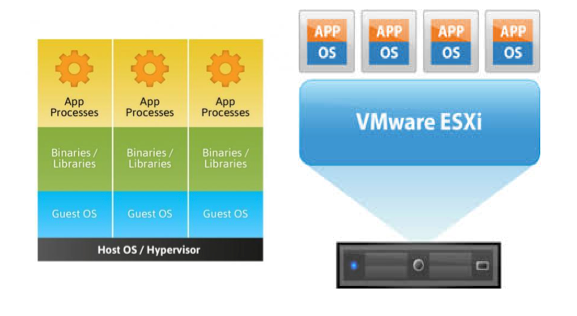
\includegraphics[width=1\textwidth]{images/virtualize-hyper.png}
  \caption
    [Virtualization based on hypervisor]
    {Virtualization based on hypervisor \cite{linuxcontainers}}
  \label{fig:virtualize-hyper}
\end{figure}

\begin{figure}[htb]\centering
  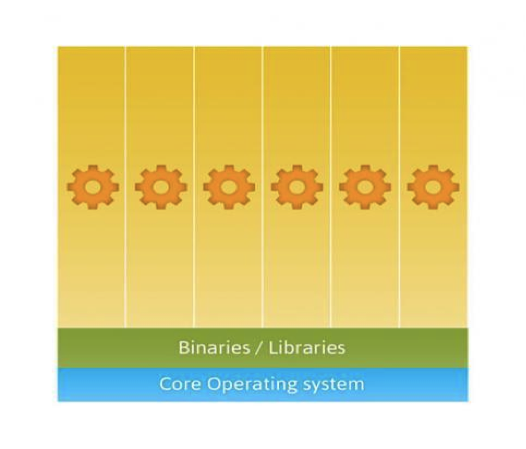
\includegraphics[width=1\textwidth]{images/virtualize-container.png}
  \caption
    [Virtualization based on containers]
    {Virtualization based on containers \cite{linuxcontainers}}
  \label{fig:virtualize-container}
\end{figure}
